\documentclass{article}[12pt]

% useful packages
\usepackage{titlesec}
\usepackage{fullpage}
\usepackage{amsmath,amssymb,amsthm,amsfonts}
\usepackage{graphicx}
\usepackage{enumerate}
\usepackage{algorithm,algorithmic}
\usepackage{xcolor}
\usepackage{bbm}
\usepackage{url}
\usepackage{hyperref}

% theorem type environments
\newtheorem{thm}{Theorem}
\newtheorem{prop}{Proposition}
\newtheorem{lemma}{Lemma}
\newtheorem{cor}{Corollary}
\newtheorem{defn}{Definition}
\newtheorem{assump}{Assumption}
\newtheorem{example}{Example}
\newtheorem{conjecture}{Conjecture}

% frequently used symbols
\newcommand{\bE}{\mathbb{E}}
\newcommand{\bP}{\mathbb{P}}
\newcommand{\bQ}{\mathbb{Q}}
\newcommand{\bR}{\mathbb{R}}
\newcommand{\bS}{\mathbb{S}}
\newcommand{\bN}{\mathbb{N}}
\newcommand{\bZ}{\mathbb{Z}}
\newcommand{\sC}{{\mathcal C}} 
\newcommand{\sD}{{\mathcal D}} 
\newcommand{\sE}{{\mathcal E}} 
\newcommand{\sF}{{\mathcal F}} 
\newcommand{\sL}{{\mathcal L}} 
\newcommand{\sH}{{\mathcal H}} 
\newcommand{\sN}{{\mathcal N}} 
\newcommand{\sO}{{\mathcal O}} 
\newcommand{\sP}{{\mathcal P}} 
\newcommand{\sR}{{\mathcal R}} 
\newcommand{\sS}{{\mathcal S}}
\newcommand{\sU}{{\mathcal U}} 
\newcommand{\sX}{{\mathcal X}} 
\newcommand{\sY}{{\mathcal Y}} 
\newcommand{\sZ}{{\mathcal Z}}

% operators
\newcommand{\sign}{\mathop{\mathrm{sign}}}
\newcommand{\supp}{\mathop{\mathrm{supp}}} % support
\newcommand{\argmin}{\operatornamewithlimits{arg\ min}}
\newcommand{\argmax}{\operatornamewithlimits{arg\ max}}
\newcommand{\dist}{\operatorname{dist}}
\newcommand{\tr}{\text{tr}}
\newcommand{\vecop}{\text{vec}}
\newcommand{\st}{\operatorname{s.t.}}
\newcommand{\cut}{\setminus}
\newcommand{\ind}[1]{\mathbbm{1}\left\{#1\right\}} 
\newcommand{\given}{\ | \ }

% grouping operators
\newcommand{\brac}[1]{\left[#1\right]}
\newcommand{\set}[1]{\left\{#1\right\}}
\newcommand{\abs}[1]{\left\lvert #1 \right\rvert}
\newcommand{\paren}[1]{\left(#1\right)}
\newcommand{\norm}[1]{\left\|#1\right\|}
\newcommand{\ip}[2]{\left\langle #1,#2 \right\rangle}

% code commands
\newcommand{\matlab}{\textsc{Matlab }}
\newcommand{\python}{\textsc{Python }}
\newcommand{\todo}[1]{\textcolor{red}{#1}}

% header command
\newcommand{\project}[3]{
    \pagestyle{myheadings}
    \thispagestyle{plain}
    \newpage
    \setcounter{page}{1}
    \setlength{\headsep}{10mm}
    \noindent
    \begin{center}
    \framebox{
        \vbox{\vspace{2mm}
            \hbox to 6.28in { {\bf EE 519: Deep Learning Theory \& Fundamentals
            \hfill Spring \the\year} }
        \vspace{4mm}
        \hbox to 6.28in { {\Large \hfill Mini Project #1 \hfill} }
        \vspace{2mm}
        \hbox to 6.28in { \Large \hfill Due: #2, 11:59PM PT \hfill }
        \vspace{2mm}
        \hbox to 6.28in { {\it Student Name: #3} \hfill {\it Instructor Name: John Lipor}}
        \vspace{2mm}}
   }
   \end{center}
   \markboth{Mini Project #1}{Mini Project #1}
   \vspace*{4mm}
}

\begin{document}

% PUT YOUR NAME BELOW WHERE I HAVE \X
\project{1}{April 28, \the\year}{Andy Franck}
% PUT YOUR NAME ABOVE WHERE I HAVE \X

\section*{Problem Description}

\indent
The objective of this project is to first train a Convolutional Neural Network capable of accurately categorizing geothermal heat flow residuals into one of four disctinct classes. After categorizing, the model will be studied using guided backpropogation to determine whether the trained model is utilizing certain structural settings to make its predictions (i.e. changes in elevation and topography). \\
\indent
The model will be trained on a detrended elevation map, partitioned into 222, 200x200 pixel images. For each patch, the label is the maximum residual value among all wells in the patch. The data is provided by the United States Geological Survey \cite{USGS}. \\
\indent
Although it would be convenient for the model to accurately predict a high percentage of labels, it is unlikely to happen with the limited data size. This report aims to develop a model that can accurately predict the labels with a reasonable degree of accuracy, and then analyze the model's behavior to determine whether it is utilizing the desired structural features to make its predictions.\\
\indent
Even without perfect model accuracy, the model can still be useful in determining what topographic features are most useful for predicting geothermal heat flow. This will lead to a better understanding of the relationship between topography and geothermal heat flow, and will help to inform future research.\\


\section*{Exploratory Data Analysis}

Because of the nature of the data, it was not necessary to perform much data analysis. It was easy to load directly from the files, and straightforward to work with through both the PyTorch and Numpy libraries. \\
\indent
To begin, the image data values were considered, and it was noted that many did not lie in the range $[0,255]$. Because of this, the image data was normalized, which resulted in a slight ~1.2\% increase in accuracy aftr training the model. The data ranges are shown below:

\begin{center}
    \begin{tabular}{|c|c|c|}
        Range & min & max \\
        Before Normalization & -1037.89 & 2596.36 \\
        After Normalization & -0.3997 & 1 \\
    \end{tabular}
\end{center}

\indent
After normalizing all of the image data, a few different image augmentation methods were considered, all from the torchvision.transforms library \cite{transforms}. Note that all data image transforms are performed inside of the training loop for each dataloader iteration, so it is difficult to determine the exact size increase for the dataset. However, because the augmentation transform was placed inside of the training loop, it was possible to train the model for more epochs without overfitting on the same exact data.\\
\indent
The first method of data augmentation was to randomly apply horizontal and vertical flips to the images. This was done to increase the data size, and to make the model more robust to different orientations of the same topography.\\
\begin{center}
    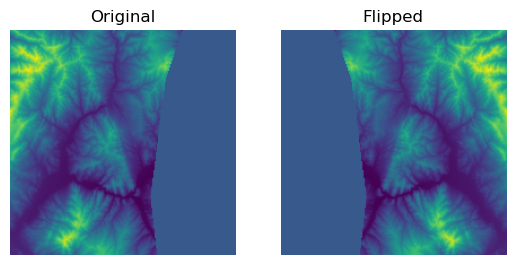
\includegraphics[width=0.5\textwidth]{images/flipped.png}
\end{center}
\indent
Secondly, the images were rotated a random amount between 0 and 90 degrees, in another effort to increase data size and increase robustness. Random Gaussian image noise was also applied to the images, but was removed after causing performance issues with little to no accuracy benefit.\\
\begin{center}
    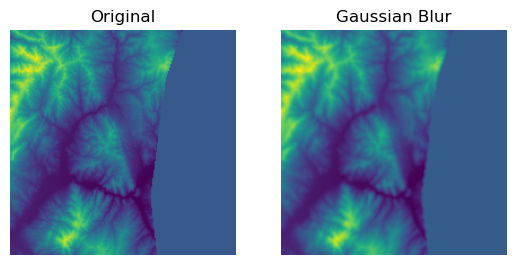
\includegraphics[width=0.5\textwidth]{images/gauss_blur.png}\\
\end{center}
\indent
Finally, the dataset contained some images that contained very little data. These images were negatively impacting the model's ability to learn, since they lacked the topographical structure that the model aimed to study. These images were removed from the dataset. This resulted in an average 2.3\% increase in accuracy. Examples are shown below:\\

\begin{center}
    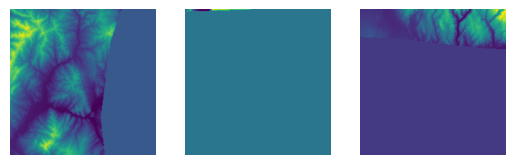
\includegraphics[width=1\textwidth]{images/low_data.png}
\end{center}

\section*{Challenges}

\indent
The largest challenge of the project was the limited data size. With only 222 images, it was very difficult to make a model train properly and accurately predict labels.\\
\indent
Additionally, the model was extremely prone to overfitting the data. To combat this, dropout was added after each Network in Network block. This helped to reduce the overfitting, however the more dropout added, the less the model seemed to learn. Unfortunately, this led to a model either overfit the data considerably, or barely learned anything at all.\\
\indent
Finally, the guided backpropogation analysis proved very difficult to implement. After adding hooks for the ReLU layers in the model, the analysis was subject to the "vanishing gradient" issue. This was solved by utilizing a different method to calculate saliency maps, without directly hooking the ReLU functions \cite{saliency}.\\



\section*{Approach}

\indent
The initial step in devlopment involved creating a baseline Network in Network model as described in the d2l textbook \cite{d2l}. This initial model was used to determine whether the data was being processed correctly, and to establish a learning baseline to be built upon. This model was trained for 100 epochs, and overfit the data considerably: \\

\begin{center}
    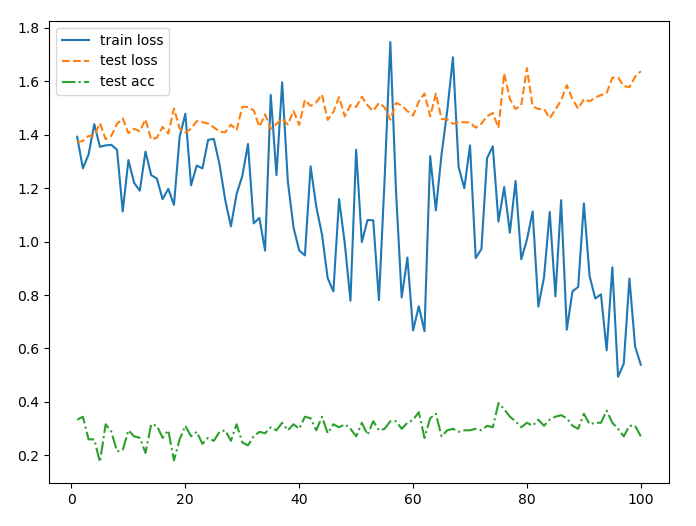
\includegraphics[width=0.5\textwidth]{images/basic_model.png}
\end{center}

\indent
The model also did not appear to be learning very well at all. This was likely due to the small data size.\\
\indent
To artifically increase the data size, image augmentation was utilized via the torchvision.transforms library \cite{transforms}. This library allows for the creation of a transform object that can be applied to a dataset. The transform object contained both random flips and rotations at random degrees. The transform was applied after loading each batch at the start of the training loop, so that each batch was augmented differently. After applying the transform, the model appeared to train slightly better, but still did not appear to be learning very well:\\
\begin{center}
    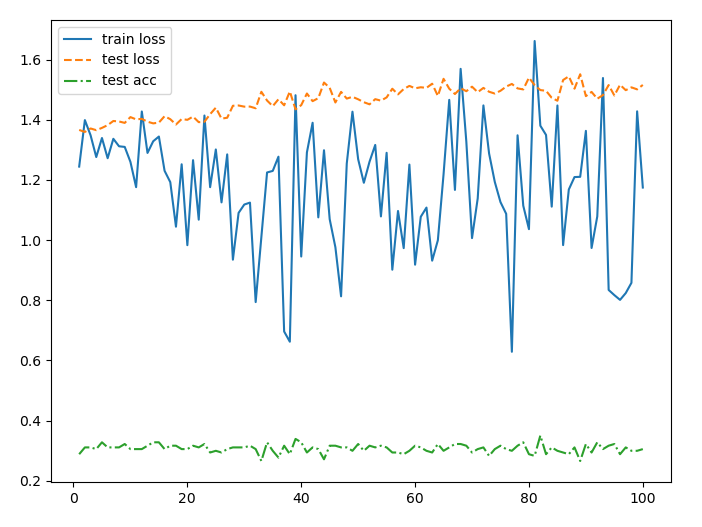
\includegraphics[width=0.5\textwidth]{images/basic_model_augmented.png}
\end{center}
The model still appeared to be overfitting, so dropout was added after each Network in Network block. This helped to reduce the overfitting, however the model did not improve in accuracy much:\\
\begin{center}
    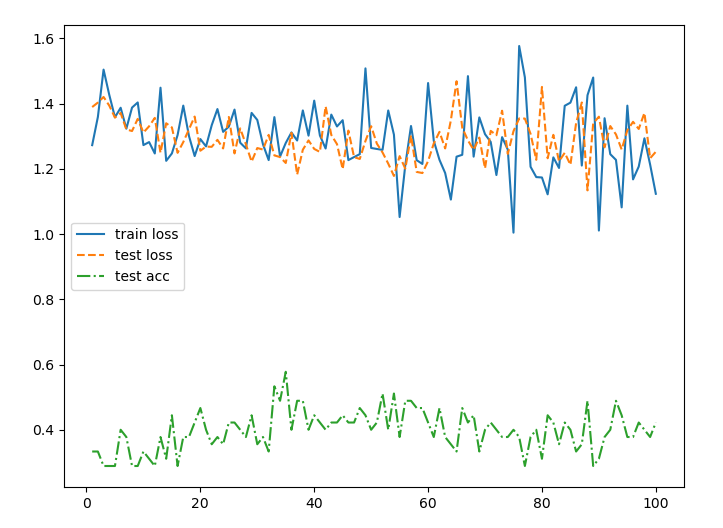
\includegraphics[width=0.5\textwidth]{images/model_augmented_dropout.png}
\end{center}
\indent
Because of the lack of data, it was decided that increasing the complexity of the model would not be benificial. The final model appears as follows, and was trained for 100 epochs at a 0.01 learning rate:\\

\begin{center}
    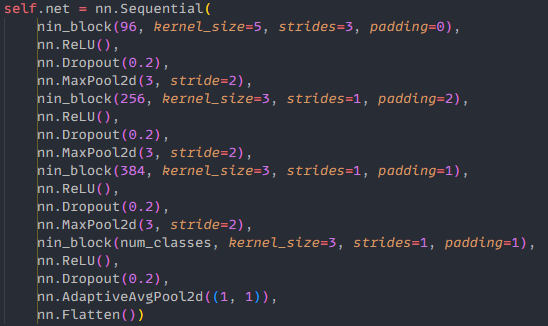
\includegraphics[width=0.5\textwidth]{images/model_code.png}
\end{center}

% Therefore, the model was kept as-is and was trained for 100 epochs. The final accuracy was 37\% over all four classes, and 66\% for binary classification. The model was then saved and used for the guided backpropogation analysis.\\
\indent
Saliency maps of the model were generated using guided backpropogation, following the tutorial \cite{saliency} and \cite{backprop}. Originally, a hook was added to every ReLU activation layer in the network, and then the model was run on a single image. The gradients were then calculated at the output layer with respect to the input image. However, this method resulted in many gradient values equal to zero, so a modification was made following \cite{saliency} to calculate the gradients without directly hooking the ReLU layers.\\

\section*{Evaluation and Summary}

Unfortunately, the model did not have a high accuracy. The final accuracy was 37\% over all four classes, and 66\% for binary classification.\\

\indent


\section*{What I Learned}

This project was an excellent introduction to image processing using convolutional neural networks. Having already developed basic models to analyze features, this project was a great way to delve deeper into more complex neural network methods. This project also involved more freedoms in regards to choice of neural network design. In the prior project, hyperparameter optimization libraries were used that made most of the experiementation unnecessary.\\
\indent
Additionally, this project served as a great introduction to image specific data modification methods. The torchvision.transforms library \cite{transforms} was very useful in this regard, and it was interesting to see how the data augmentation methods affected the model's ability to learn.\\
\indent
Finally, this project was a great introduction to guided backpropogation. This method was very useful in determining which features the model was utilizing to make its predictions, and a great introduction to more advanced machine learning techniques. Tutorials such as \cite{saliency}, \cite{backprop} were invaluable for developing a better understanding on hooking the model and calculating the gradients.\\

\bibliographystyle{IEEEtran}
\bibliography{bibliography}

\end{document}